\documentclass[12pt,letterpaper]{article}
\usepackage[margin=0.65in,top=0.75in,bottom=0.65in,headheight=15pt,headsep=17pt,footskip=24pt]{geometry}
\usepackage{lmodern}
\pdfmapfile{+lm.map}
\pdfmapfile{+cm.map}
\usepackage{tikz}
\usetikzlibrary{arrows.meta}
\usepackage{fancyhdr}
\renewcommand{\familydefault}{\sfdefault}
\setlength{\parindent}{0pt}
\setlength{\parskip}{7pt}
\pagestyle{fancy}
\fancyhf{}
\renewcommand{\headrulewidth}{0pt}
\renewcommand{\footrulewidth}{0pt}
\fancyhead[L]{\fontsize{11}{13}\selectfont Week 13 / Route packing and bottlenecks / K--1}
\fancyfoot[L]{\fontsize{9}{11}\selectfont Bellingham Math Circle / Week 13 / F13-K-v2}
\fancyfoot[R]{\fontsize{9}{11}\selectfont\thepage}
\begin{document}
\fontsize{14}{18}\selectfont
A route follows arrows from Start to Finish without visiting a dot twice. Routes may meet at dots, but each arrow can belong to only one route in a collection. Use a different color or line pattern for each route. A marker closes one arrow.
\vspace{0.1in}
\par\textbf{Problem 1:} Fit as many routes as you can on each board. Find another largest collection, if you can.

\vspace{0.05in}
\begin{center}
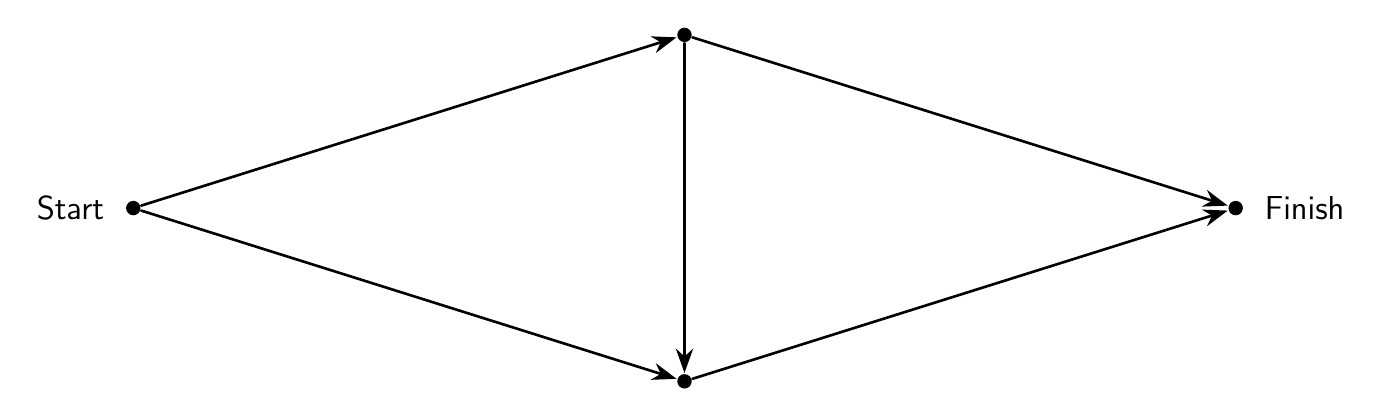
\begin{tikzpicture}[x=1cm,y=1cm,>={Stealth[length=3.1mm,width=2.2mm]},line cap=round,line join=round]
\coordinate (s) at (0,0);
\coordinate (A) at (7,2.2);
\coordinate (B) at (7,-2.2);
\coordinate (t) at (14,0);
\draw[->,line width=0.95pt,shorten >=3pt,shorten <=3pt] (s) -- (A);
\draw[->,line width=0.95pt,shorten >=3pt,shorten <=3pt] (s) -- (B);
\draw[->,line width=0.95pt,shorten >=3pt,shorten <=3pt] (A) -- (B);
\draw[->,line width=0.95pt,shorten >=3pt,shorten <=3pt] (A) -- (t);
\draw[->,line width=0.95pt,shorten >=3pt,shorten <=3pt] (B) -- (t);
\fill (s) circle (2.6pt);
\node[left=7pt,font=\fontsize{12}{14}\selectfont] at (s) {Start};
\fill (A) circle (2.6pt);
\fill (B) circle (2.6pt);
\fill (t) circle (2.6pt);
\node[right=7pt,font=\fontsize{12}{14}\selectfont] at (t) {Finish};
\end{tikzpicture}
\end{center}
\vspace{0.32in}
\begin{center}
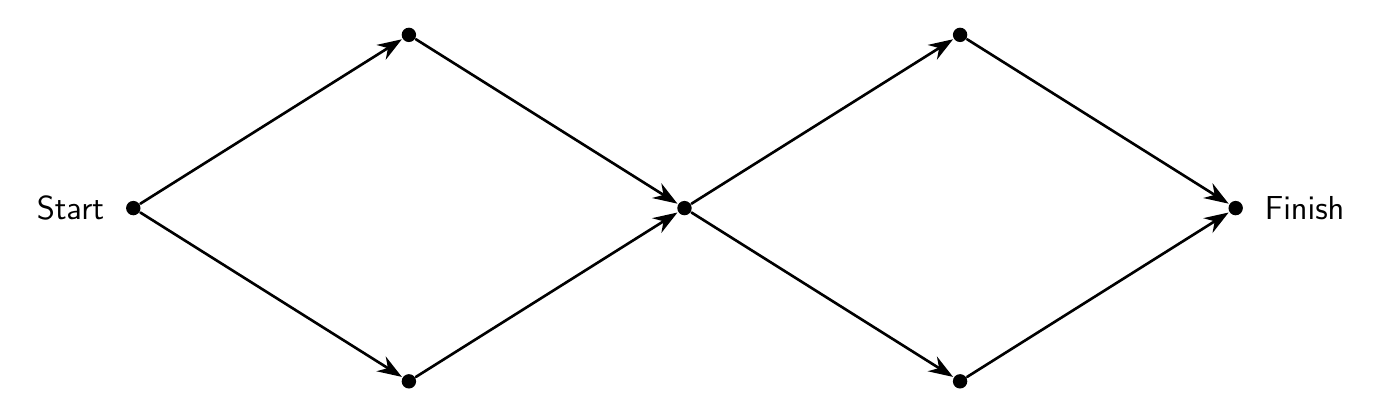
\begin{tikzpicture}[x=1cm,y=1cm,>={Stealth[length=3.1mm,width=2.2mm]},line cap=round,line join=round]
\coordinate (s) at (0,0);
\coordinate (A) at (3.5,2.2);
\coordinate (B) at (3.5,-2.2);
\coordinate (C) at (7,0);
\coordinate (D) at (10.5,2.2);
\coordinate (E) at (10.5,-2.2);
\coordinate (t) at (14,0);
\draw[->,line width=0.95pt,shorten >=3pt,shorten <=3pt] (s) -- (A);
\draw[->,line width=0.95pt,shorten >=3pt,shorten <=3pt] (s) -- (B);
\draw[->,line width=0.95pt,shorten >=3pt,shorten <=3pt] (A) -- (C);
\draw[->,line width=0.95pt,shorten >=3pt,shorten <=3pt] (B) -- (C);
\draw[->,line width=0.95pt,shorten >=3pt,shorten <=3pt] (C) -- (D);
\draw[->,line width=0.95pt,shorten >=3pt,shorten <=3pt] (C) -- (E);
\draw[->,line width=0.95pt,shorten >=3pt,shorten <=3pt] (D) -- (t);
\draw[->,line width=0.95pt,shorten >=3pt,shorten <=3pt] (E) -- (t);
\fill (s) circle (2.6pt);
\node[left=7pt,font=\fontsize{12}{14}\selectfont] at (s) {Start};
\fill (A) circle (2.6pt);
\fill (B) circle (2.6pt);
\fill (C) circle (2.6pt);
\fill (D) circle (2.6pt);
\fill (E) circle (2.6pt);
\fill (t) circle (2.6pt);
\node[right=7pt,font=\fontsize{12}{14}\selectfont] at (t) {Finish};
\end{tikzpicture}
\end{center}


\newpage
\par\textbf{Problem 2:} Stop every route with as few markers as you can. Find another way with the same number of markers, if you can.

\vspace{0.26in}
\begin{center}
\begin{tikzpicture}[x=1cm,y=1cm,>={Stealth[length=3.1mm,width=2.2mm]},line cap=round,line join=round]
\coordinate (s) at (0,0);
\coordinate (A) at (7,2.2);
\coordinate (B) at (7,-2.2);
\coordinate (t) at (14,0);
\draw[->,line width=0.95pt,shorten >=3pt,shorten <=3pt] (s) -- (A);
\draw[->,line width=0.95pt,shorten >=3pt,shorten <=3pt] (s) -- (B);
\draw[->,line width=0.95pt,shorten >=3pt,shorten <=3pt] (A) -- (t);
\draw[->,line width=0.95pt,shorten >=3pt,shorten <=3pt] (B) -- (t);
\fill (s) circle (2.6pt);
\node[left=7pt,font=\fontsize{12}{14}\selectfont] at (s) {Start};
\fill (A) circle (2.6pt);
\fill (B) circle (2.6pt);
\fill (t) circle (2.6pt);
\node[right=7pt,font=\fontsize{12}{14}\selectfont] at (t) {Finish};
\end{tikzpicture}
\end{center}
\vspace{0.32in}
\begin{center}
\begin{tikzpicture}[x=1cm,y=1cm,>={Stealth[length=3.1mm,width=2.2mm]},line cap=round,line join=round]
\coordinate (s) at (0,0);
\coordinate (A) at (3,2.2);
\coordinate (B) at (3,-2.2);
\coordinate (C) at (6,0);
\coordinate (D) at (9,0);
\coordinate (t) at (14,0);
\draw[->,line width=0.95pt,shorten >=3pt,shorten <=3pt] (s) -- (A);
\draw[->,line width=0.95pt,shorten >=3pt,shorten <=3pt] (s) -- (B);
\draw[->,line width=0.95pt,shorten >=3pt,shorten <=3pt] (A) -- (C);
\draw[->,line width=0.95pt,shorten >=3pt,shorten <=3pt] (B) -- (C);
\draw[->,line width=0.95pt,shorten >=3pt,shorten <=3pt] (C) -- (D);
\draw[->,line width=0.95pt,shorten >=3pt,shorten <=3pt] (D) -- (t);
\fill (s) circle (2.6pt);
\node[left=7pt,font=\fontsize{12}{14}\selectfont] at (s) {Start};
\fill (A) circle (2.6pt);
\fill (B) circle (2.6pt);
\fill (C) circle (2.6pt);
\fill (D) circle (2.6pt);
\fill (t) circle (2.6pt);
\node[right=7pt,font=\fontsize{12}{14}\selectfont] at (t) {Finish};
\end{tikzpicture}
\end{center}


\newpage
\par\textbf{Problem 3:} Fit the most routes on each board. Then stop all travel with the same number of markers.

\vspace{0.26in}
\begin{center}
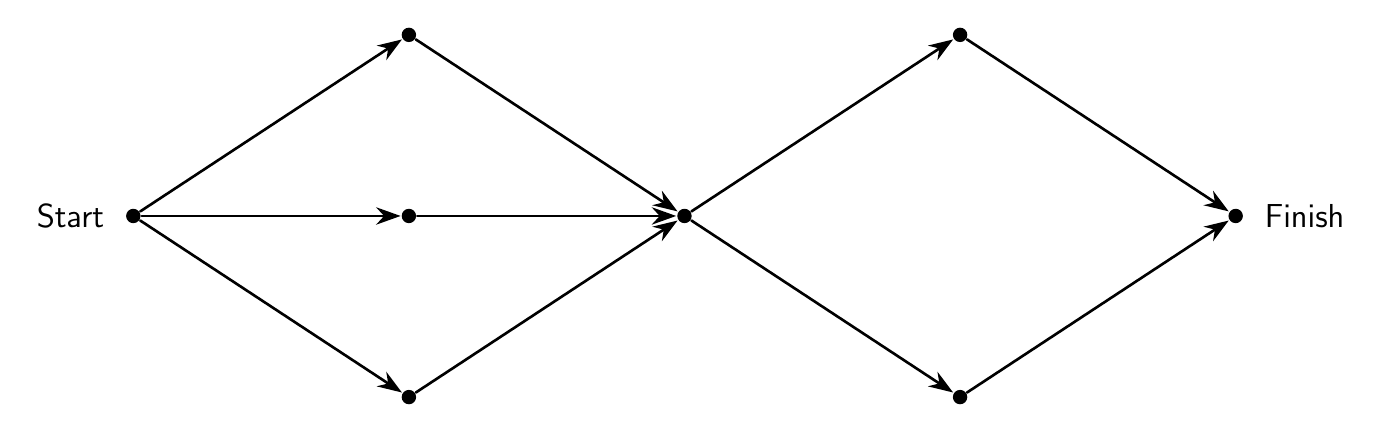
\begin{tikzpicture}[x=1cm,y=1cm,>={Stealth[length=3.1mm,width=2.2mm]},line cap=round,line join=round]
\coordinate (s) at (0,0);
\coordinate (A) at (3.5,2.3);
\coordinate (B) at (3.5,0);
\coordinate (C) at (3.5,-2.3);
\coordinate (D) at (7,0);
\coordinate (E) at (10.5,2.3);
\coordinate (F) at (10.5,-2.3);
\coordinate (t) at (14,0);
\draw[->,line width=0.95pt,shorten >=3pt,shorten <=3pt] (s) -- (A);
\draw[->,line width=0.95pt,shorten >=3pt,shorten <=3pt] (s) -- (B);
\draw[->,line width=0.95pt,shorten >=3pt,shorten <=3pt] (s) -- (C);
\draw[->,line width=0.95pt,shorten >=3pt,shorten <=3pt] (A) -- (D);
\draw[->,line width=0.95pt,shorten >=3pt,shorten <=3pt] (B) -- (D);
\draw[->,line width=0.95pt,shorten >=3pt,shorten <=3pt] (C) -- (D);
\draw[->,line width=0.95pt,shorten >=3pt,shorten <=3pt] (D) -- (E);
\draw[->,line width=0.95pt,shorten >=3pt,shorten <=3pt] (D) -- (F);
\draw[->,line width=0.95pt,shorten >=3pt,shorten <=3pt] (E) -- (t);
\draw[->,line width=0.95pt,shorten >=3pt,shorten <=3pt] (F) -- (t);
\fill (s) circle (2.6pt);
\node[left=7pt,font=\fontsize{12}{14}\selectfont] at (s) {Start};
\fill (A) circle (2.6pt);
\fill (B) circle (2.6pt);
\fill (C) circle (2.6pt);
\fill (D) circle (2.6pt);
\fill (E) circle (2.6pt);
\fill (F) circle (2.6pt);
\fill (t) circle (2.6pt);
\node[right=7pt,font=\fontsize{12}{14}\selectfont] at (t) {Finish};
\end{tikzpicture}
\end{center}
\vspace{0.32in}
\begin{center}
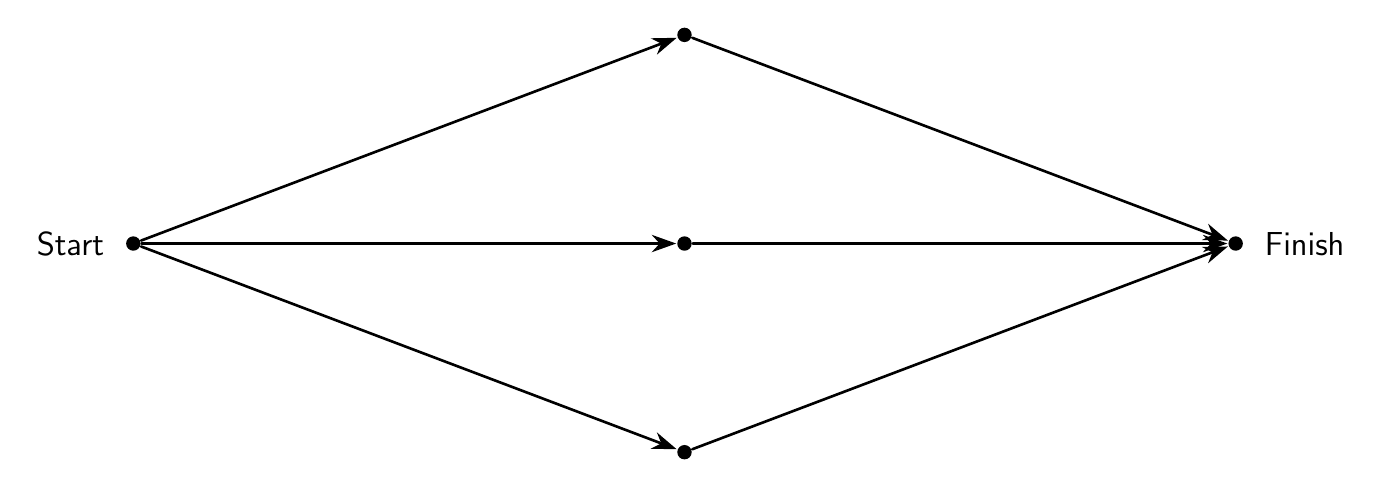
\begin{tikzpicture}[x=1cm,y=1cm,>={Stealth[length=3.1mm,width=2.2mm]},line cap=round,line join=round]
\coordinate (s) at (0,0);
\coordinate (A) at (7,2.65);
\coordinate (B) at (7,0);
\coordinate (C) at (7,-2.65);
\coordinate (t) at (14,0);
\draw[->,line width=0.95pt,shorten >=3pt,shorten <=3pt] (s) -- (A);
\draw[->,line width=0.95pt,shorten >=3pt,shorten <=3pt] (s) -- (B);
\draw[->,line width=0.95pt,shorten >=3pt,shorten <=3pt] (s) -- (C);
\draw[->,line width=0.95pt,shorten >=3pt,shorten <=3pt] (A) -- (t);
\draw[->,line width=0.95pt,shorten >=3pt,shorten <=3pt] (B) -- (t);
\draw[->,line width=0.95pt,shorten >=3pt,shorten <=3pt] (C) -- (t);
\fill (s) circle (2.6pt);
\node[left=7pt,font=\fontsize{12}{14}\selectfont] at (s) {Start};
\fill (A) circle (2.6pt);
\fill (B) circle (2.6pt);
\fill (C) circle (2.6pt);
\fill (t) circle (2.6pt);
\node[right=7pt,font=\fontsize{12}{14}\selectfont] at (t) {Finish};
\end{tikzpicture}
\end{center}


\newpage
\par\textbf{Problem 4:} Close just one arrow at a time. Find every arrow you could close and still fit two routes.

\vspace{0.26in}
\begin{center}
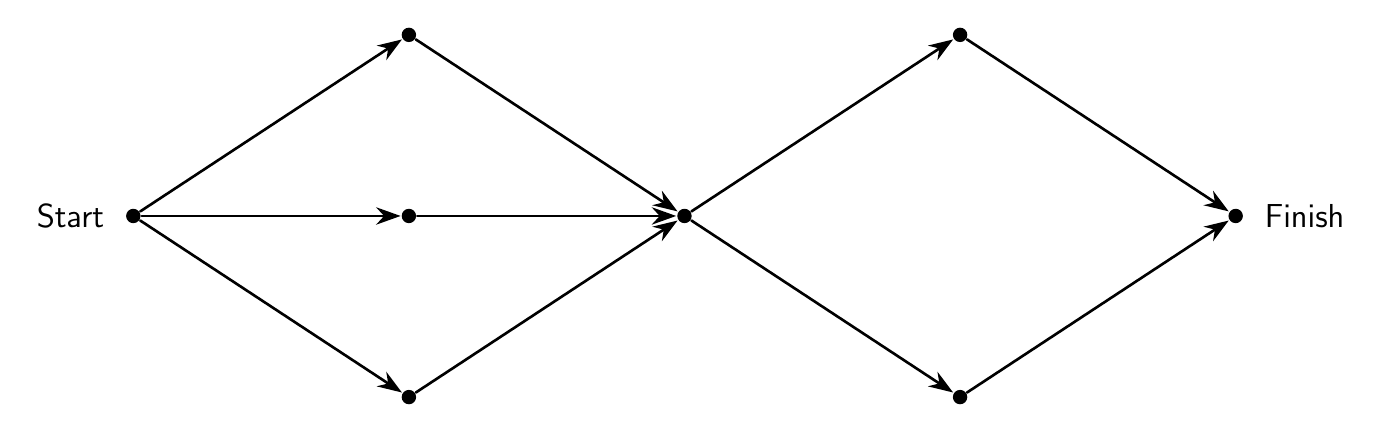
\begin{tikzpicture}[x=1cm,y=1cm,>={Stealth[length=3.1mm,width=2.2mm]},line cap=round,line join=round]
\coordinate (s) at (0,0);
\coordinate (A) at (3.5,2.3);
\coordinate (B) at (3.5,0);
\coordinate (C) at (3.5,-2.3);
\coordinate (D) at (7,0);
\coordinate (E) at (10.5,2.3);
\coordinate (F) at (10.5,-2.3);
\coordinate (t) at (14,0);
\draw[->,line width=0.95pt,shorten >=3pt,shorten <=3pt] (s) -- (A);
\draw[->,line width=0.95pt,shorten >=3pt,shorten <=3pt] (s) -- (B);
\draw[->,line width=0.95pt,shorten >=3pt,shorten <=3pt] (s) -- (C);
\draw[->,line width=0.95pt,shorten >=3pt,shorten <=3pt] (A) -- (D);
\draw[->,line width=0.95pt,shorten >=3pt,shorten <=3pt] (B) -- (D);
\draw[->,line width=0.95pt,shorten >=3pt,shorten <=3pt] (C) -- (D);
\draw[->,line width=0.95pt,shorten >=3pt,shorten <=3pt] (D) -- (E);
\draw[->,line width=0.95pt,shorten >=3pt,shorten <=3pt] (D) -- (F);
\draw[->,line width=0.95pt,shorten >=3pt,shorten <=3pt] (E) -- (t);
\draw[->,line width=0.95pt,shorten >=3pt,shorten <=3pt] (F) -- (t);
\fill (s) circle (2.6pt);
\node[left=7pt,font=\fontsize{12}{14}\selectfont] at (s) {Start};
\fill (A) circle (2.6pt);
\fill (B) circle (2.6pt);
\fill (C) circle (2.6pt);
\fill (D) circle (2.6pt);
\fill (E) circle (2.6pt);
\fill (F) circle (2.6pt);
\fill (t) circle (2.6pt);
\node[right=7pt,font=\fontsize{12}{14}\selectfont] at (t) {Finish};
\end{tikzpicture}
\end{center}
\vspace{0.32in}
\begin{center}
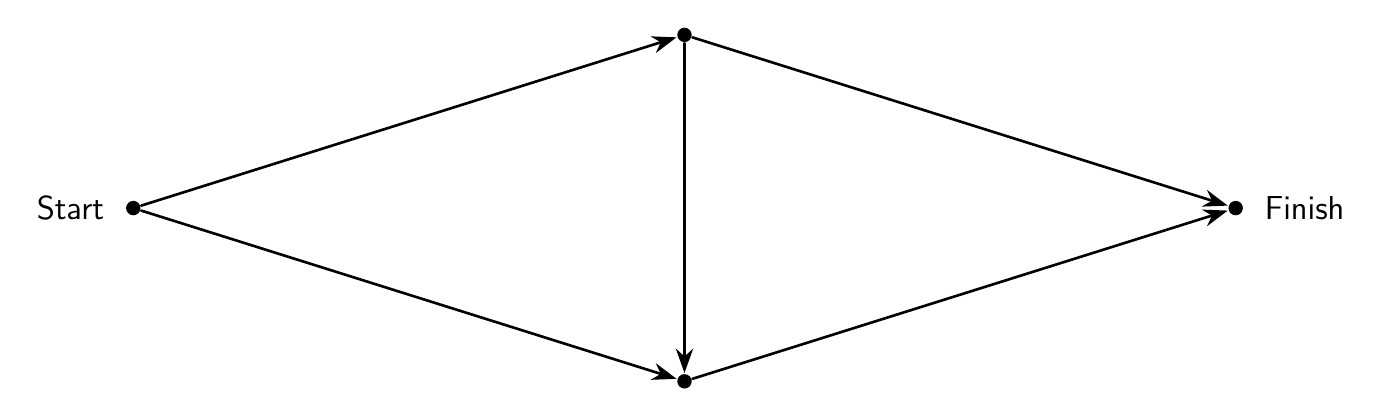
\begin{tikzpicture}[x=1cm,y=1cm,>={Stealth[length=3.1mm,width=2.2mm]},line cap=round,line join=round]
\coordinate (s) at (0,0);
\coordinate (A) at (7,2.2);
\coordinate (B) at (7,-2.2);
\coordinate (t) at (14,0);
\draw[->,line width=0.95pt,shorten >=3pt,shorten <=3pt] (s) -- (A);
\draw[->,line width=0.95pt,shorten >=3pt,shorten <=3pt] (s) -- (B);
\draw[->,line width=0.95pt,shorten >=3pt,shorten <=3pt] (A) -- (B);
\draw[->,line width=0.95pt,shorten >=3pt,shorten <=3pt] (A) -- (t);
\draw[->,line width=0.95pt,shorten >=3pt,shorten <=3pt] (B) -- (t);
\fill (s) circle (2.6pt);
\node[left=7pt,font=\fontsize{12}{14}\selectfont] at (s) {Start};
\fill (A) circle (2.6pt);
\fill (B) circle (2.6pt);
\fill (t) circle (2.6pt);
\node[right=7pt,font=\fontsize{12}{14}\selectfont] at (t) {Finish};
\end{tikzpicture}
\end{center}


\newpage
\par\textbf{Problem 5:} Stop every route with two markers. Find every different pair of arrows that works.

\vspace{0.08in}
\begin{center}
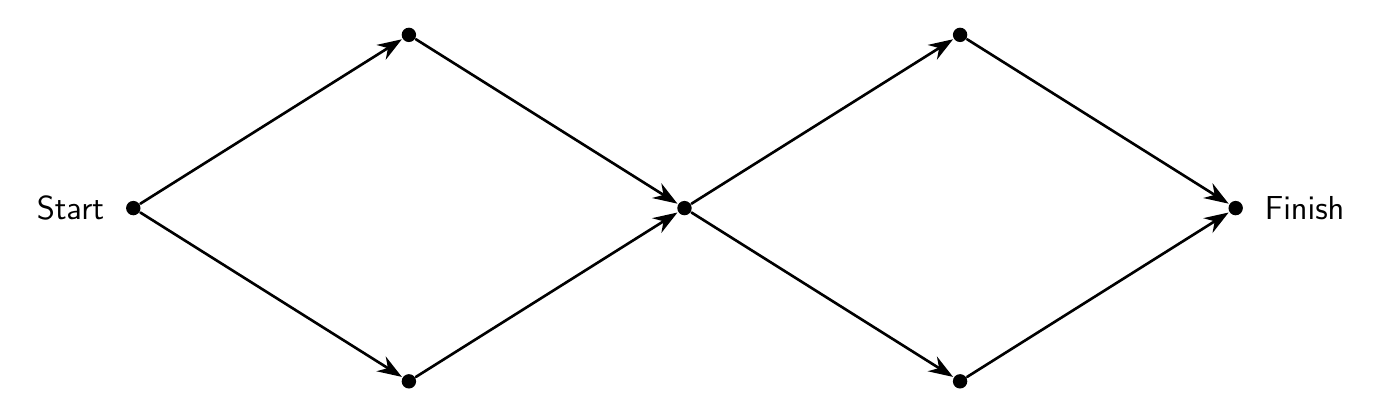
\begin{tikzpicture}[x=1cm,y=1cm,>={Stealth[length=3.1mm,width=2.2mm]},line cap=round,line join=round]
\coordinate (s) at (0,0);
\coordinate (A) at (3.5,2.2);
\coordinate (B) at (3.5,-2.2);
\coordinate (C) at (7,0);
\coordinate (D) at (10.5,2.2);
\coordinate (E) at (10.5,-2.2);
\coordinate (t) at (14,0);
\draw[->,line width=0.95pt,shorten >=3pt,shorten <=3pt] (s) -- (A);
\draw[->,line width=0.95pt,shorten >=3pt,shorten <=3pt] (s) -- (B);
\draw[->,line width=0.95pt,shorten >=3pt,shorten <=3pt] (A) -- (C);
\draw[->,line width=0.95pt,shorten >=3pt,shorten <=3pt] (B) -- (C);
\draw[->,line width=0.95pt,shorten >=3pt,shorten <=3pt] (C) -- (D);
\draw[->,line width=0.95pt,shorten >=3pt,shorten <=3pt] (C) -- (E);
\draw[->,line width=0.95pt,shorten >=3pt,shorten <=3pt] (D) -- (t);
\draw[->,line width=0.95pt,shorten >=3pt,shorten <=3pt] (E) -- (t);
\fill (s) circle (2.6pt);
\node[left=7pt,font=\fontsize{12}{14}\selectfont] at (s) {Start};
\fill (A) circle (2.6pt);
\fill (B) circle (2.6pt);
\fill (C) circle (2.6pt);
\fill (D) circle (2.6pt);
\fill (E) circle (2.6pt);
\fill (t) circle (2.6pt);
\node[right=7pt,font=\fontsize{12}{14}\selectfont] at (t) {Finish};
\end{tikzpicture}
\end{center}
\vspace{0.08in}
\noindent\begin{minipage}{0.48\linewidth}\centering
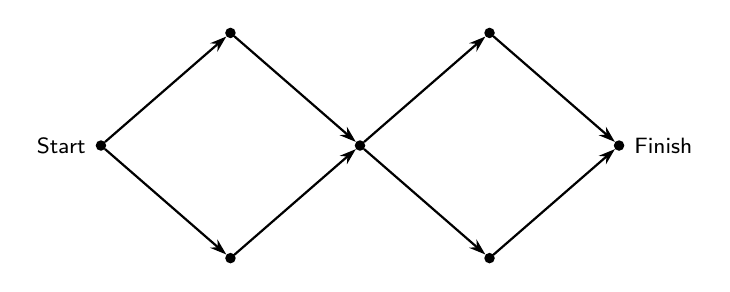
\begin{tikzpicture}[x=0.47cm,y=0.65cm,>={Stealth[length=2.1mm,width=1.4mm]},line cap=round,line join=round]
\coordinate (s) at (0,0);
\coordinate (A) at (3.5,2.2);
\coordinate (B) at (3.5,-2.2);
\coordinate (C) at (7,0);
\coordinate (D) at (10.5,2.2);
\coordinate (E) at (10.5,-2.2);
\coordinate (t) at (14,0);
\draw[->,line width=0.8pt,shorten >=2pt,shorten <=2pt] (s) -- (A);
\draw[->,line width=0.8pt,shorten >=2pt,shorten <=2pt] (s) -- (B);
\draw[->,line width=0.8pt,shorten >=2pt,shorten <=2pt] (A) -- (C);
\draw[->,line width=0.8pt,shorten >=2pt,shorten <=2pt] (B) -- (C);
\draw[->,line width=0.8pt,shorten >=2pt,shorten <=2pt] (C) -- (D);
\draw[->,line width=0.8pt,shorten >=2pt,shorten <=2pt] (C) -- (E);
\draw[->,line width=0.8pt,shorten >=2pt,shorten <=2pt] (D) -- (t);
\draw[->,line width=0.8pt,shorten >=2pt,shorten <=2pt] (E) -- (t);
\fill (s) circle (1.9pt);
\node[left=2pt,font=\fontsize{8}{9}\selectfont] at (s) {Start};
\fill (A) circle (1.9pt);
\fill (B) circle (1.9pt);
\fill (C) circle (1.9pt);
\fill (D) circle (1.9pt);
\fill (E) circle (1.9pt);
\fill (t) circle (1.9pt);
\node[right=2pt,font=\fontsize{8}{9}\selectfont] at (t) {Finish};
\end{tikzpicture}\end{minipage}\hfill\begin{minipage}{0.48\linewidth}\centering
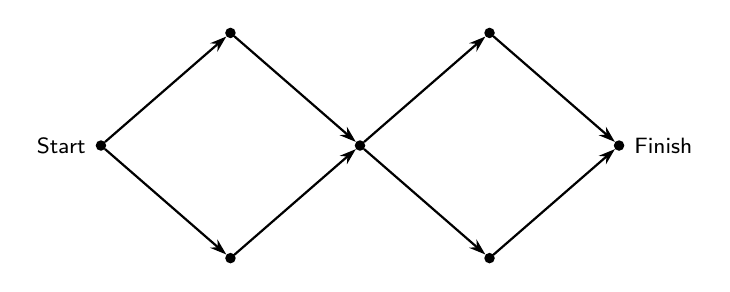
\begin{tikzpicture}[x=0.47cm,y=0.65cm,>={Stealth[length=2.1mm,width=1.4mm]},line cap=round,line join=round]
\coordinate (s) at (0,0);
\coordinate (A) at (3.5,2.2);
\coordinate (B) at (3.5,-2.2);
\coordinate (C) at (7,0);
\coordinate (D) at (10.5,2.2);
\coordinate (E) at (10.5,-2.2);
\coordinate (t) at (14,0);
\draw[->,line width=0.8pt,shorten >=2pt,shorten <=2pt] (s) -- (A);
\draw[->,line width=0.8pt,shorten >=2pt,shorten <=2pt] (s) -- (B);
\draw[->,line width=0.8pt,shorten >=2pt,shorten <=2pt] (A) -- (C);
\draw[->,line width=0.8pt,shorten >=2pt,shorten <=2pt] (B) -- (C);
\draw[->,line width=0.8pt,shorten >=2pt,shorten <=2pt] (C) -- (D);
\draw[->,line width=0.8pt,shorten >=2pt,shorten <=2pt] (C) -- (E);
\draw[->,line width=0.8pt,shorten >=2pt,shorten <=2pt] (D) -- (t);
\draw[->,line width=0.8pt,shorten >=2pt,shorten <=2pt] (E) -- (t);
\fill (s) circle (1.9pt);
\node[left=2pt,font=\fontsize{8}{9}\selectfont] at (s) {Start};
\fill (A) circle (1.9pt);
\fill (B) circle (1.9pt);
\fill (C) circle (1.9pt);
\fill (D) circle (1.9pt);
\fill (E) circle (1.9pt);
\fill (t) circle (1.9pt);
\node[right=2pt,font=\fontsize{8}{9}\selectfont] at (t) {Finish};
\end{tikzpicture}\end{minipage}
\par\vspace{0.15in}
\noindent\begin{minipage}{0.48\linewidth}\centering
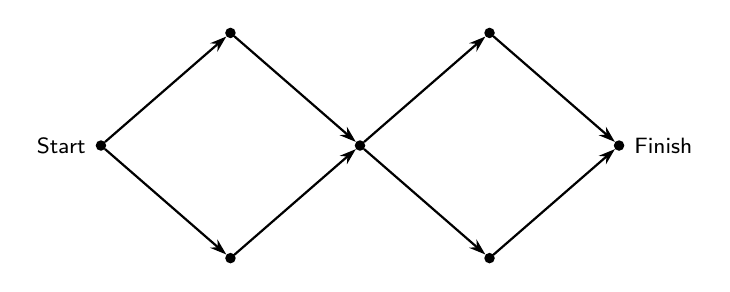
\begin{tikzpicture}[x=0.47cm,y=0.65cm,>={Stealth[length=2.1mm,width=1.4mm]},line cap=round,line join=round]
\coordinate (s) at (0,0);
\coordinate (A) at (3.5,2.2);
\coordinate (B) at (3.5,-2.2);
\coordinate (C) at (7,0);
\coordinate (D) at (10.5,2.2);
\coordinate (E) at (10.5,-2.2);
\coordinate (t) at (14,0);
\draw[->,line width=0.8pt,shorten >=2pt,shorten <=2pt] (s) -- (A);
\draw[->,line width=0.8pt,shorten >=2pt,shorten <=2pt] (s) -- (B);
\draw[->,line width=0.8pt,shorten >=2pt,shorten <=2pt] (A) -- (C);
\draw[->,line width=0.8pt,shorten >=2pt,shorten <=2pt] (B) -- (C);
\draw[->,line width=0.8pt,shorten >=2pt,shorten <=2pt] (C) -- (D);
\draw[->,line width=0.8pt,shorten >=2pt,shorten <=2pt] (C) -- (E);
\draw[->,line width=0.8pt,shorten >=2pt,shorten <=2pt] (D) -- (t);
\draw[->,line width=0.8pt,shorten >=2pt,shorten <=2pt] (E) -- (t);
\fill (s) circle (1.9pt);
\node[left=2pt,font=\fontsize{8}{9}\selectfont] at (s) {Start};
\fill (A) circle (1.9pt);
\fill (B) circle (1.9pt);
\fill (C) circle (1.9pt);
\fill (D) circle (1.9pt);
\fill (E) circle (1.9pt);
\fill (t) circle (1.9pt);
\node[right=2pt,font=\fontsize{8}{9}\selectfont] at (t) {Finish};
\end{tikzpicture}\end{minipage}\hfill\begin{minipage}{0.48\linewidth}\centering
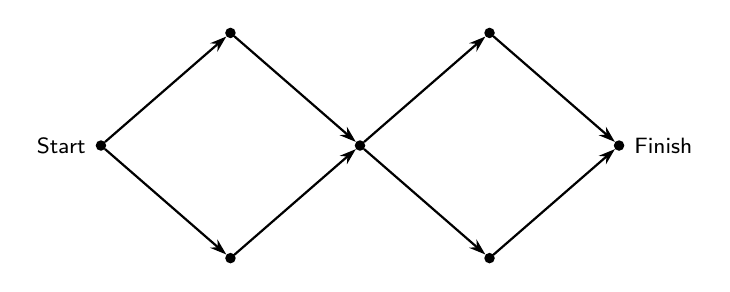
\begin{tikzpicture}[x=0.47cm,y=0.65cm,>={Stealth[length=2.1mm,width=1.4mm]},line cap=round,line join=round]
\coordinate (s) at (0,0);
\coordinate (A) at (3.5,2.2);
\coordinate (B) at (3.5,-2.2);
\coordinate (C) at (7,0);
\coordinate (D) at (10.5,2.2);
\coordinate (E) at (10.5,-2.2);
\coordinate (t) at (14,0);
\draw[->,line width=0.8pt,shorten >=2pt,shorten <=2pt] (s) -- (A);
\draw[->,line width=0.8pt,shorten >=2pt,shorten <=2pt] (s) -- (B);
\draw[->,line width=0.8pt,shorten >=2pt,shorten <=2pt] (A) -- (C);
\draw[->,line width=0.8pt,shorten >=2pt,shorten <=2pt] (B) -- (C);
\draw[->,line width=0.8pt,shorten >=2pt,shorten <=2pt] (C) -- (D);
\draw[->,line width=0.8pt,shorten >=2pt,shorten <=2pt] (C) -- (E);
\draw[->,line width=0.8pt,shorten >=2pt,shorten <=2pt] (D) -- (t);
\draw[->,line width=0.8pt,shorten >=2pt,shorten <=2pt] (E) -- (t);
\fill (s) circle (1.9pt);
\node[left=2pt,font=\fontsize{8}{9}\selectfont] at (s) {Start};
\fill (A) circle (1.9pt);
\fill (B) circle (1.9pt);
\fill (C) circle (1.9pt);
\fill (D) circle (1.9pt);
\fill (E) circle (1.9pt);
\fill (t) circle (1.9pt);
\node[right=2pt,font=\fontsize{8}{9}\selectfont] at (t) {Finish};
\end{tikzpicture}\end{minipage}
\par\vspace{0.15in}
\noindent\begin{minipage}{0.48\linewidth}\centering
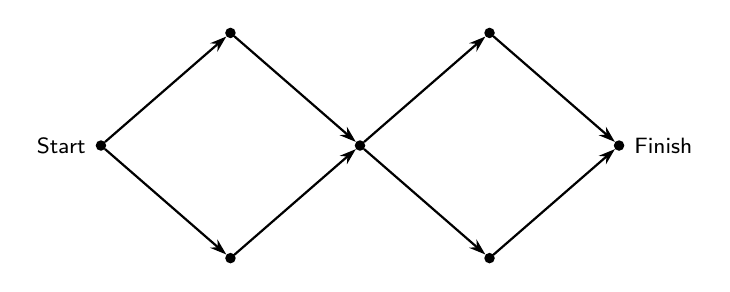
\begin{tikzpicture}[x=0.47cm,y=0.65cm,>={Stealth[length=2.1mm,width=1.4mm]},line cap=round,line join=round]
\coordinate (s) at (0,0);
\coordinate (A) at (3.5,2.2);
\coordinate (B) at (3.5,-2.2);
\coordinate (C) at (7,0);
\coordinate (D) at (10.5,2.2);
\coordinate (E) at (10.5,-2.2);
\coordinate (t) at (14,0);
\draw[->,line width=0.8pt,shorten >=2pt,shorten <=2pt] (s) -- (A);
\draw[->,line width=0.8pt,shorten >=2pt,shorten <=2pt] (s) -- (B);
\draw[->,line width=0.8pt,shorten >=2pt,shorten <=2pt] (A) -- (C);
\draw[->,line width=0.8pt,shorten >=2pt,shorten <=2pt] (B) -- (C);
\draw[->,line width=0.8pt,shorten >=2pt,shorten <=2pt] (C) -- (D);
\draw[->,line width=0.8pt,shorten >=2pt,shorten <=2pt] (C) -- (E);
\draw[->,line width=0.8pt,shorten >=2pt,shorten <=2pt] (D) -- (t);
\draw[->,line width=0.8pt,shorten >=2pt,shorten <=2pt] (E) -- (t);
\fill (s) circle (1.9pt);
\node[left=2pt,font=\fontsize{8}{9}\selectfont] at (s) {Start};
\fill (A) circle (1.9pt);
\fill (B) circle (1.9pt);
\fill (C) circle (1.9pt);
\fill (D) circle (1.9pt);
\fill (E) circle (1.9pt);
\fill (t) circle (1.9pt);
\node[right=2pt,font=\fontsize{8}{9}\selectfont] at (t) {Finish};
\end{tikzpicture}\end{minipage}\hfill\begin{minipage}{0.48\linewidth}\centering
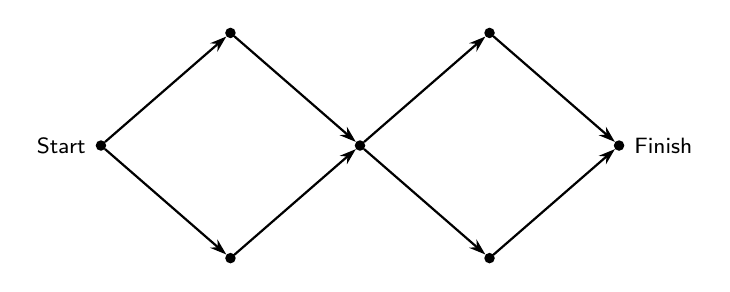
\begin{tikzpicture}[x=0.47cm,y=0.65cm,>={Stealth[length=2.1mm,width=1.4mm]},line cap=round,line join=round]
\coordinate (s) at (0,0);
\coordinate (A) at (3.5,2.2);
\coordinate (B) at (3.5,-2.2);
\coordinate (C) at (7,0);
\coordinate (D) at (10.5,2.2);
\coordinate (E) at (10.5,-2.2);
\coordinate (t) at (14,0);
\draw[->,line width=0.8pt,shorten >=2pt,shorten <=2pt] (s) -- (A);
\draw[->,line width=0.8pt,shorten >=2pt,shorten <=2pt] (s) -- (B);
\draw[->,line width=0.8pt,shorten >=2pt,shorten <=2pt] (A) -- (C);
\draw[->,line width=0.8pt,shorten >=2pt,shorten <=2pt] (B) -- (C);
\draw[->,line width=0.8pt,shorten >=2pt,shorten <=2pt] (C) -- (D);
\draw[->,line width=0.8pt,shorten >=2pt,shorten <=2pt] (C) -- (E);
\draw[->,line width=0.8pt,shorten >=2pt,shorten <=2pt] (D) -- (t);
\draw[->,line width=0.8pt,shorten >=2pt,shorten <=2pt] (E) -- (t);
\fill (s) circle (1.9pt);
\node[left=2pt,font=\fontsize{8}{9}\selectfont] at (s) {Start};
\fill (A) circle (1.9pt);
\fill (B) circle (1.9pt);
\fill (C) circle (1.9pt);
\fill (D) circle (1.9pt);
\fill (E) circle (1.9pt);
\fill (t) circle (1.9pt);
\node[right=2pt,font=\fontsize{8}{9}\selectfont] at (t) {Finish};
\end{tikzpicture}\end{minipage}
\par\vspace{0.15in}
\noindent\begin{minipage}{0.48\linewidth}\centering
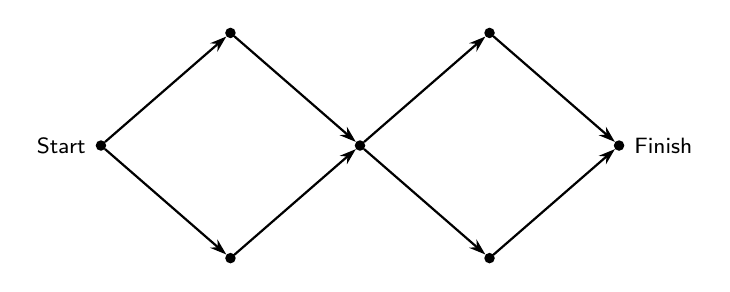
\begin{tikzpicture}[x=0.47cm,y=0.65cm,>={Stealth[length=2.1mm,width=1.4mm]},line cap=round,line join=round]
\coordinate (s) at (0,0);
\coordinate (A) at (3.5,2.2);
\coordinate (B) at (3.5,-2.2);
\coordinate (C) at (7,0);
\coordinate (D) at (10.5,2.2);
\coordinate (E) at (10.5,-2.2);
\coordinate (t) at (14,0);
\draw[->,line width=0.8pt,shorten >=2pt,shorten <=2pt] (s) -- (A);
\draw[->,line width=0.8pt,shorten >=2pt,shorten <=2pt] (s) -- (B);
\draw[->,line width=0.8pt,shorten >=2pt,shorten <=2pt] (A) -- (C);
\draw[->,line width=0.8pt,shorten >=2pt,shorten <=2pt] (B) -- (C);
\draw[->,line width=0.8pt,shorten >=2pt,shorten <=2pt] (C) -- (D);
\draw[->,line width=0.8pt,shorten >=2pt,shorten <=2pt] (C) -- (E);
\draw[->,line width=0.8pt,shorten >=2pt,shorten <=2pt] (D) -- (t);
\draw[->,line width=0.8pt,shorten >=2pt,shorten <=2pt] (E) -- (t);
\fill (s) circle (1.9pt);
\node[left=2pt,font=\fontsize{8}{9}\selectfont] at (s) {Start};
\fill (A) circle (1.9pt);
\fill (B) circle (1.9pt);
\fill (C) circle (1.9pt);
\fill (D) circle (1.9pt);
\fill (E) circle (1.9pt);
\fill (t) circle (1.9pt);
\node[right=2pt,font=\fontsize{8}{9}\selectfont] at (t) {Finish};
\end{tikzpicture}\end{minipage}\hfill\begin{minipage}{0.48\linewidth}\centering
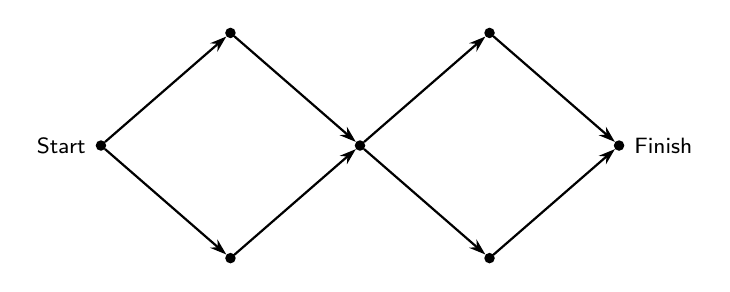
\begin{tikzpicture}[x=0.47cm,y=0.65cm,>={Stealth[length=2.1mm,width=1.4mm]},line cap=round,line join=round]
\coordinate (s) at (0,0);
\coordinate (A) at (3.5,2.2);
\coordinate (B) at (3.5,-2.2);
\coordinate (C) at (7,0);
\coordinate (D) at (10.5,2.2);
\coordinate (E) at (10.5,-2.2);
\coordinate (t) at (14,0);
\draw[->,line width=0.8pt,shorten >=2pt,shorten <=2pt] (s) -- (A);
\draw[->,line width=0.8pt,shorten >=2pt,shorten <=2pt] (s) -- (B);
\draw[->,line width=0.8pt,shorten >=2pt,shorten <=2pt] (A) -- (C);
\draw[->,line width=0.8pt,shorten >=2pt,shorten <=2pt] (B) -- (C);
\draw[->,line width=0.8pt,shorten >=2pt,shorten <=2pt] (C) -- (D);
\draw[->,line width=0.8pt,shorten >=2pt,shorten <=2pt] (C) -- (E);
\draw[->,line width=0.8pt,shorten >=2pt,shorten <=2pt] (D) -- (t);
\draw[->,line width=0.8pt,shorten >=2pt,shorten <=2pt] (E) -- (t);
\fill (s) circle (1.9pt);
\node[left=2pt,font=\fontsize{8}{9}\selectfont] at (s) {Start};
\fill (A) circle (1.9pt);
\fill (B) circle (1.9pt);
\fill (C) circle (1.9pt);
\fill (D) circle (1.9pt);
\fill (E) circle (1.9pt);
\fill (t) circle (1.9pt);
\node[right=2pt,font=\fontsize{8}{9}\selectfont] at (t) {Finish};
\end{tikzpicture}\end{minipage}

\newpage
\par\textbf{Problem 6:} Two players take turns closing one open arrow; whoever leaves no route wins. On each board, would you rather go first or second, and how can you win?

\vspace{0.26in}
\begin{center}
\begin{tikzpicture}[x=1cm,y=1cm,>={Stealth[length=3.1mm,width=2.2mm]},line cap=round,line join=round]
\coordinate (s) at (0,0);
\coordinate (A) at (7,2.2);
\coordinate (B) at (7,-2.2);
\coordinate (t) at (14,0);
\draw[->,line width=0.95pt,shorten >=3pt,shorten <=3pt] (s) -- (A);
\draw[->,line width=0.95pt,shorten >=3pt,shorten <=3pt] (s) -- (B);
\draw[->,line width=0.95pt,shorten >=3pt,shorten <=3pt] (A) -- (t);
\draw[->,line width=0.95pt,shorten >=3pt,shorten <=3pt] (B) -- (t);
\fill (s) circle (2.6pt);
\node[left=7pt,font=\fontsize{12}{14}\selectfont] at (s) {Start};
\fill (A) circle (2.6pt);
\fill (B) circle (2.6pt);
\fill (t) circle (2.6pt);
\node[right=7pt,font=\fontsize{12}{14}\selectfont] at (t) {Finish};
\end{tikzpicture}
\end{center}
\vspace{0.32in}
\begin{center}
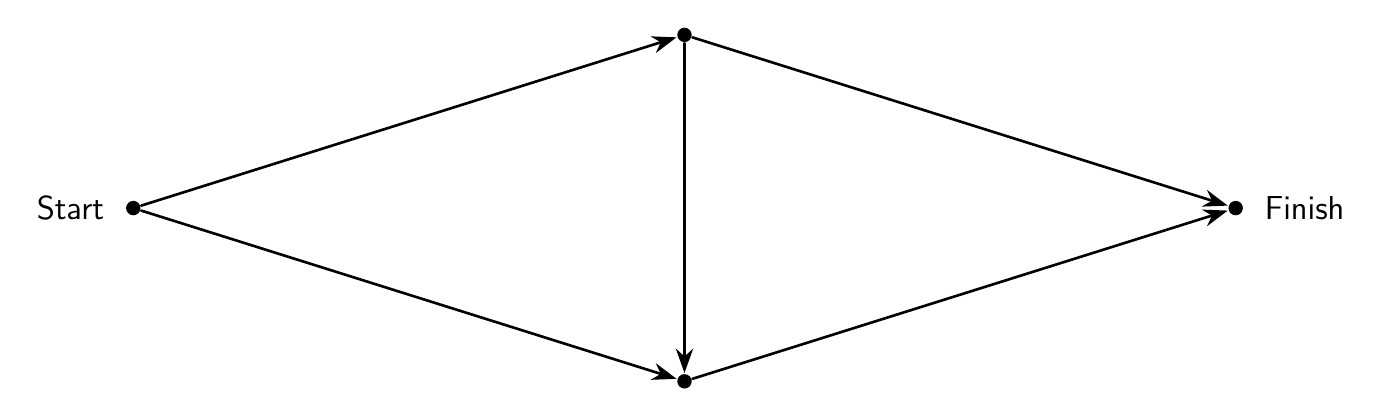
\begin{tikzpicture}[x=1cm,y=1cm,>={Stealth[length=3.1mm,width=2.2mm]},line cap=round,line join=round]
\coordinate (s) at (0,0);
\coordinate (A) at (7,2.2);
\coordinate (B) at (7,-2.2);
\coordinate (t) at (14,0);
\draw[->,line width=0.95pt,shorten >=3pt,shorten <=3pt] (s) -- (A);
\draw[->,line width=0.95pt,shorten >=3pt,shorten <=3pt] (s) -- (B);
\draw[->,line width=0.95pt,shorten >=3pt,shorten <=3pt] (A) -- (B);
\draw[->,line width=0.95pt,shorten >=3pt,shorten <=3pt] (A) -- (t);
\draw[->,line width=0.95pt,shorten >=3pt,shorten <=3pt] (B) -- (t);
\fill (s) circle (2.6pt);
\node[left=7pt,font=\fontsize{12}{14}\selectfont] at (s) {Start};
\fill (A) circle (2.6pt);
\fill (B) circle (2.6pt);
\fill (t) circle (2.6pt);
\node[right=7pt,font=\fontsize{12}{14}\selectfont] at (t) {Finish};
\end{tikzpicture}
\end{center}


\end{document}
